%!TEX root=masterproef.tex

\chapter{Architectuur}
\label{chapter:architectuur}

De oplossingsstrategie stelt voor om een uitwendige DSL te combineren met code
generatie om zo een volledig geautomatiseerde keten te bekomen van onderzoek
tot uitbating. Dit hoofdstuk bekijkt de oplossing vanuit een architectuur
oogpunt.

Sectie \ref{section:arch-functional} bekijkt de functionaliteit van de
oplossing en identificeert de verschillende functionele componenten met hun
onderlinge relaties. Dit overzicht identificeert tevens de scope die zal
aangehouden worden in het vervolg van deze masterproef.

Sectie \ref{section:arch-technical} werkt vervolgens deze functionele uit in
een technische architectuur. Hier wordt het functionele proces opgedeeld in
technische componenten en worden de verschillende interne informatiestromen,
-manipulaties en -opslagvormen.

\section{Functionele architectuur}
\label{section:arch-functional}

Figuur \ref{fig:arch-functional} geeft een overzicht van de voorgestelde
oplossing.

\begin{figure}[ht]
  \centering
  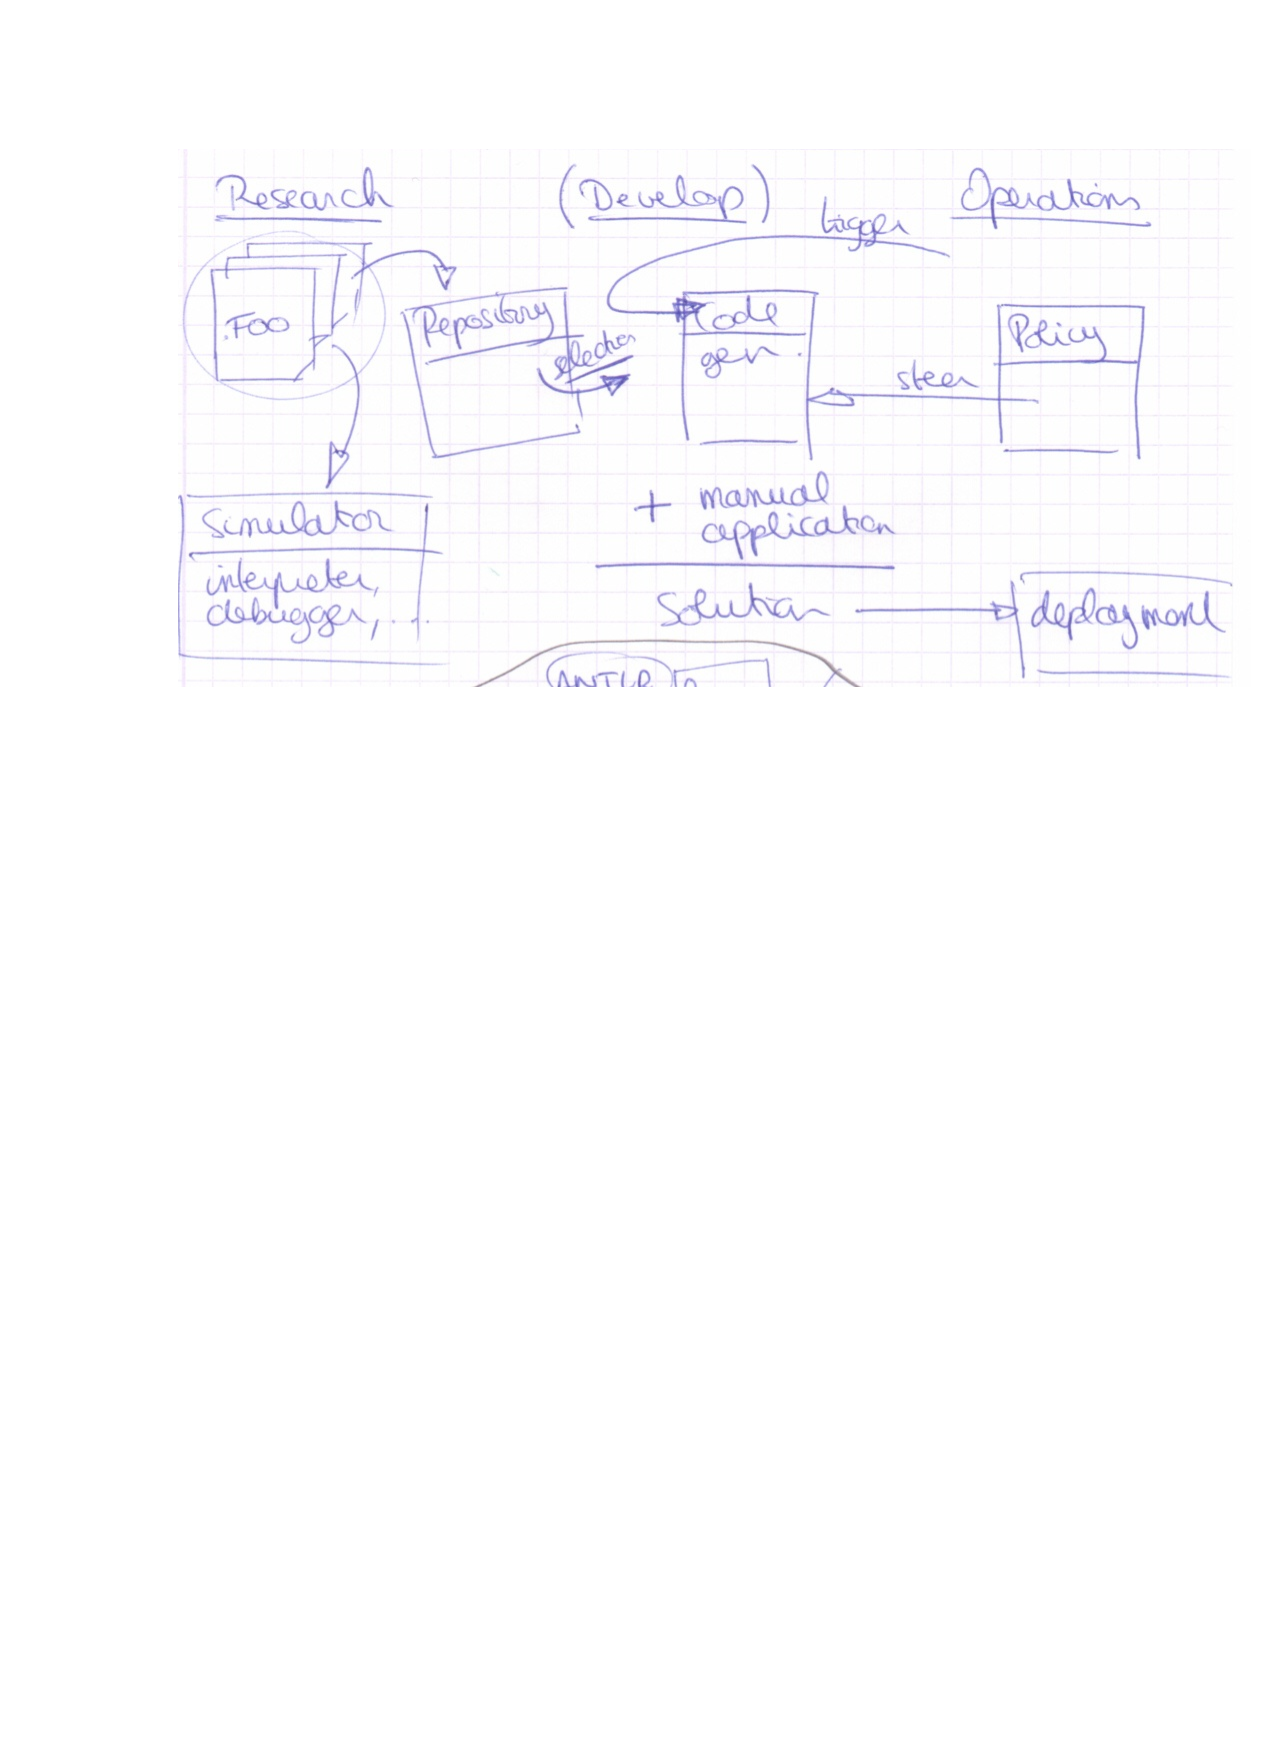
\includegraphics[width=0.9\linewidth]{resources/arch-functional.pdf}
  \caption{Functionele architectuur}
  \label{fig:arch-functional}
\end{figure}

\subsection{FOO-lang}
\label{subsection:arch-foo-lang}

De eerste belangrijke component van de oplossing is de domeinspecifieke taal,
waarmee detectiealgoritmen kunnen beschreven worden. De belangrijkste
doelstelling van de taal is om de functionaliteit zo optimaal mogelijk te
organiseren. Hierdoor wordt getracht om het gebruik van de \mcu en het gebruik
van de draadloze radio te beperken. Deze doelstelling wordt ook weerspiegeld in
de naam: Functie Organisatie Optimalisatie (\emph{Function Organisation
Optimisation}), kortweg: FOO-lang.

De belangrijkste doelgroep wat betreft gebruikers, zijn onderzoekers van IDS in
WSN. Met FOO-lang kunnen zij beschikken over een formele taal om
inbraakdetectiealgoritmen voor WSN te beschrijven.

Het is van primordiaal belang dat de taal zo dicht mogelijk aansluit bij
bestaande kennis en vertrouwde paradigma. Daarom wordt voorgesteld om dicht bij
de C programmeertaal aan te blijven leunen en deze uit te breiden met niet
ongewone constructies om het niveau van de taal op een hoger niveau van
abstractie te brengen. Dit hogere niveau sluit meer aan bij een functionele en
platform-onafhankelijke beschrijving.

Om de doelstelling na te streven is het belangrijk dat er control is over de
iteratieve aspecten van de algoritmen. Deze gaan typisch om de sensorknopen in
de nabijheid van de knoop in kwestie. Door de functionaliteit van het domein te
centraliseren rond deze knopen, is het mogelijk om deze iteraties weg te
werken. Door het defini\"eren van gebeurtenissen waarop kan gereageerd worden
met functionaliteit, is het mogelijk om abstractie te maken van de volledige
lijst van sensorknopen en het algoritme in stukken te breken die als reacties
op de gebeurtenissen kunnen beschreven worden.

Om het functionele karakter verder te onderstrepen is het belangrijk dat zoveel
mogelijk technische aspecten uit de algoritmen geweerd worden. Een typische
voorbeeld is de typering van variabelen. Typering zal een noodzaak blijken,
maar moet op zijn minst optioneel zijn en indien nodig voorzien worden als een
beperkte set van functionele types. Dit is ook een belangrijke voorwaarde voor
de platform-onafhankelijkheid.

\subsection{Centrale opslag}
\label{subsection:arch-repository}

Al deze platform-onafhankelijke en formele beschrijvingen van
detectiealgoritmen, kunnen vervolgens samengebracht worden in een centrale
opslagplaats. Het hoeft geen betoog dat hiervoor een website kan voorzien
worden, die als portaal kan dienen. Een heel aantal klassieke voorzieningen
kunnen hierbij getroffen worden: zoekmogelijkheden, gebruiksstatistieken,
commentaar, samenwerkmogelijkheden \dots

Allerhande integraties kunnen voorzien worden om op transparante wijze met
zoveel mogelijk de facto standaard diensten te kunnen samenwerken. Hierbij
denken we aan diensten die opslag van programmacode aanbieden, of meer algemeen
opslag van bestanden, tot processturingsplatformen of probleemopvolgsystemen.

De toegang tot de broncode van de algoritmen moet enerzijds mogelijk zijn via
de visuele website, maar moet zeker geautomatiseerd ge\"integreerd kunnen
worden, zodat bv. compilatieprocessen de laatste versie van een algoritme
kunnen downloaden zonder tussenkomst van een persoon.

\subsection{Code generatie}
\label{subsection:arch-codegen}

Het kloppend hart van de oplossing bestaat uit de code generator. Deze
accepteert de in FOO-lang geschreven algoritmen en vormt deze om tot
georganiseerde code voor het geselecteerde platform, eventueel voor een gegeven
taal \dots

De generator moet de doelstellingen van de oplossinsstrategie implementeren en
de resulterende code op zo'n manier structureren dat deze minder impact heeft
op de werking van de sensorknoop.

Om een volledig geautomatiseerde werking toe te laten is het belangrijk dat de
aansturing van de generator in zo'n een context mogelijk is. De configuratie
van de generator moet via een bestand of aan de hand van oproepparameters
gespecificeerd kunnen worden, zonder verdere menselijke tussenkomst.

\subsection{Uitbating: beleid en verspreiding}
\label{subsection:arch-policy}

Een volledig geautomatiseerde oplossing laat toe om een uitbatingsbeleid te
introduceren op veel fijnere schaal. Het wordt immers mogelijk om zelfs per
sensorknoop een ``persoonlijk'' configuratie te gaan onderhouden, bouwen en te
verspreiden.

Hierbij komt de oplossing ook te gemoed aan bv. de nood van sommige algoritmen
om op verschillende soorten knopen verschillende functionaliteit te voorzien.
Maar vanuit een uitbatingsbeleid is dit een groot voordeel. Naast de
optimalisatie van het gebruik van de middelen van \'e\'en knoop, kan nu ook een
spreiding over verschillende knopen helpen om het gemiddeld aantal algoritmen
per knoop te verlagen en zelfs dynamisch op regelmatige tijdstippen te wijzigen.

Indien gecombineerd met voorzieningen die OTAP toelaten, kan het
gedistribueerde IDS op elk ogenblik gewijzigd worden. Tal van mogelijkheden
ontstaan zo.

\subsection{Ontwikkeling}
\label{subsection:arch-integration}

Naast het IDS is er natuurlijk nog de eigenlijke toepassing die op de
sensorknoop zal ge\"installeerd en uitgebaat worden. Ook deze moet optimaal
verwerkt kunnen worden in het samenstellingsproces.

De minimale vereisten zijn dat het generatieproces duidelijke markeringen in de
resulterende code achterlaat, zodat de integratie met de toepassingscode
mogelijk is. Deze markeringen kunnen ook voorzien worden in de vorm van
invoegdirectieven die tijdens het compilatieproces bijkomende bestanden kan
opnemen zonder verdere tussenkomst van een ontwikkelaar.

\subsection{Verdere opportuniteiten}
\label{subsection:arch-opportunities}

Met een centrale opslagplaats en een volledige geautomatiseerde code generatie
en compilatieproces, zijn tal van ondersteunende toepassingen denkbaar.

Een voorbeeld dat van groot belang kan zijn voor onderzoekers is een
gestandaardiseerde simulatieomgeving. Deze zou kunnen opgebouwd worden met de
code generator, voorzien van een implementatie voor een virtueel platform, die
bruikbare code genereert voor de simulatieomgeving. Een integratie zou kunnen
bestaan in een implementatie in Javascript, wat toelaat om de simulatie toe te
voegen aan de centrale opslagplaats en dynamisch verschillende combinaties van
algoritmen uit de centrale opslagplaats te testen voor ze te integreren in een
echte omgeving.

\subsection{Scope}
\label{subsection:arch-scope}

De voorgaande hoogniveau functionele analyse toont vooral aan dat met de
basiscomponenten veel andere opportuniteiten in bereik liggen. Het is
belangrijk om deze opportuniteiten in het vizier te houden, zodat er geen
uitgesloten worden door de implementatie.

De minimale set aan basiscomponenten zal ook in deze masterproef verder
uitgewerkt worden aan de hand van een prototype. Het betreft de code generator
met ondersteuning voor een eerste platform en programmeertaal combinatie.

\section{Technische architectuur}
\label{section:arch-technical}

Figuur \ref{fig:arch-technical} toont de vertaling van de beoogde functionele
scope naar meer technische componenten. 

\begin{figure}[ht]
  \centering
  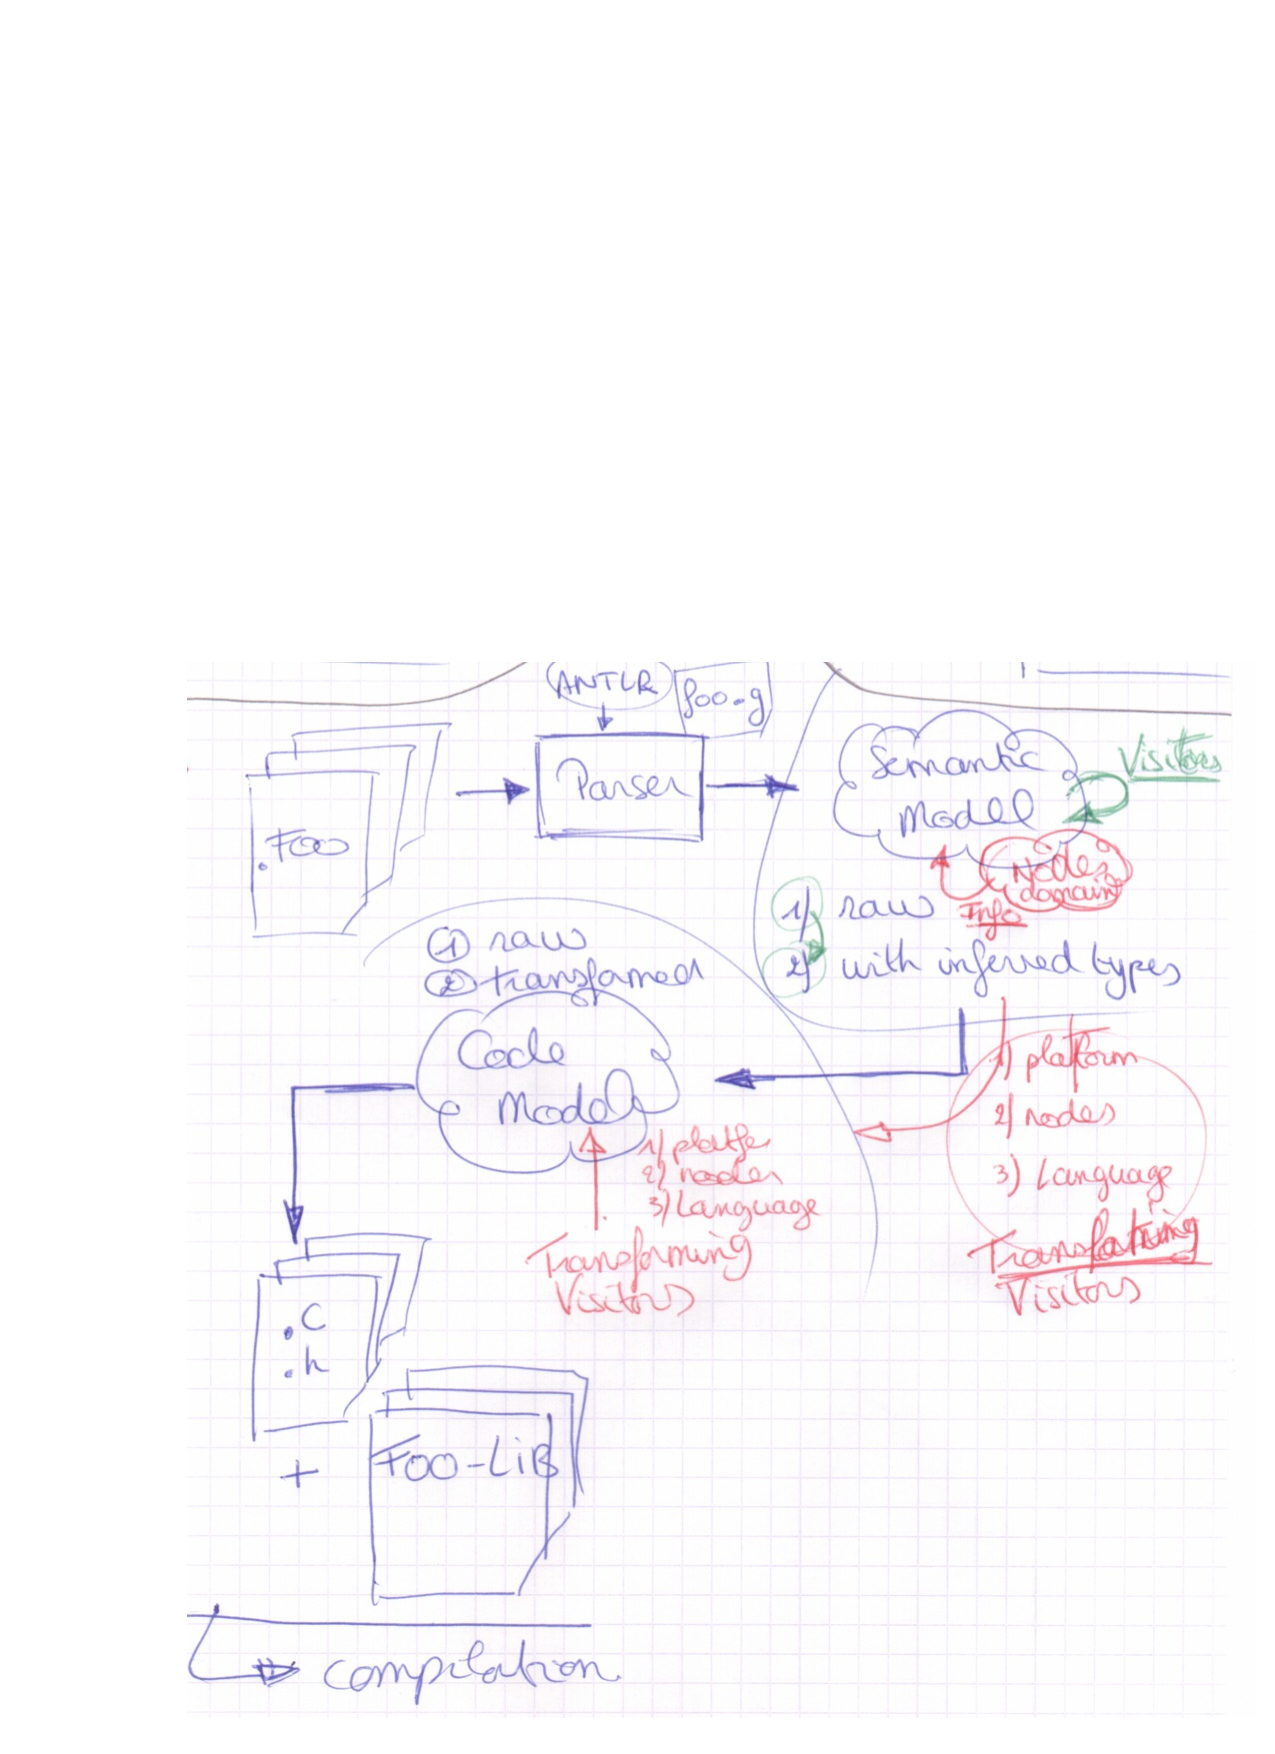
\includegraphics[width=0.9\linewidth]{resources/arch-technical.pdf}
  \caption{Technische architectuur}
  \label{fig:arch-technical}
\end{figure}

\subsection{Parser}

De verwerking verloopt als volgt: een parser analyseert de FOO-lang broncode en
produceert een zgn. abstracte syntax boomvoorstelling (\emph{Abstract
Syntax Tree} (AST). Deze AST wordt vervolgens ingeladen in een semantisch model
(SM) \citep{fowler2010domain}.

\subsection{Semantisch model}
\label{subsection:arch-semantic-model}

Een semantisch model bevat de volledige en semantisch correcte voorstelling van
de boogde functionaliteit. In die optiek vertoont het sterke overeenkomsten met
een klassiek domein model \citep{fowler2010domain}. Omdat dit laatste echter
veel rijker is aan functionaliteit en een semantisch model typisch meer
informatie-geori\"enteerd is, wordt er een onderscheid gemaakt in de naamgeving.

Het model is volledig ge\"ent op het domein waarvoor het opgebouwd wordt. In
bijlage \ref{appendix:semantic-model} wordt het SM weergegeven. Het bevat alle
functionele aspecten die nodig geacht worden om algoritmen in het domein
functioneel te beschrijven.

Op het hoogste niveau herkennen we het model als alles omvattende entiteit.
Hieronder worden de modules geplaatst, die overeenkomen met telkens \'e\'en
algoritme. Modules bevatten functionaliteit in de vorm van
functiebeschrijvingen.

Het centrale concept is dat van de uitvoeringsstrategie (Engels:
\emph{Execution Strategy})\footnote{Er is geopteerd om in de programmacode van
de generator een Engelstalige terminologie aan te houden.}. Deze verbindt
functionaliteit met de knopen. Verschillende soorten strategie\"en zijn
voorzien: een reactie op een gebeurtenis (\emph{Handler}) en een weerkerende
actie (\emph{Every}).

Op een lager niveau wordt de functionaliteit beschreven aan de hand van een
syntax die nauw aansluit bij deze van de C programmeertaal. Deze is echter wel
uitgebreid met constructies van een hoger abstractieniveau, om op een
functionelere manier om te kunnen gaan met de entiteiten uit het domein.

\subsection{Type deductie en andere transformaties}

Door middel van verschillende transformaties wordt dit SM model vervolledigd.
Een eerste stap is het deduceren van ontbrekende types. Het resultaat is een
volledig getypeerd SM en garandeert een correcte behandeling, eventueel in het
kader van een sterk getypeerde programmeertaal, zoals C.

Een tweede stap is een vertaling van het SM naar een CM. Dit CM staat dichter
bij de uiteindelijk te genereren code en meer technische van aard. Deze
vertaling is het resultaat van verschillende transformaties uitgevoerd op het
SM door de generieke code generator zelf, het platform en de domeinspecifieke
implementatie.

\subsection{Code model}
\label{subsection:arch-code-model}

Via de verschillende transformaties, wordt het SM omgezet in een CM. Deze
overstap vertaalt in essentie de functionele concepten naar overeenkomstige
patronen in een semantiek die direct aanleunt bij programmeertalen.

Het code model voorziet een hi\"erarchie van een compilatie unit, met daaronder
modules en binnen elke module secties. Dit is een abstracte voorstelling van
respectievelijk de gehele compilatie, de functionele modules en de bestanden
waaruit die modules opgebouwd zullen worden. In termen van de C programmeertaal
is dit het geheel van C en aanverwante bestanden, het concept van een C module
en op het laagste niveau de effectieve C en hoofding bestanden.

Een sectie bestaat dan uit \'e\'en of meerdere code constructies: functie
declaraties, expressies, statements \dots Deze code constructies zijn rijker
dan bv. de C programmeertaal. Het zal de taak zijn van opeenvolgende
transformaties om deze niet-gekende constructies voor een bepaald platform
en/of programmeertaal om te vormen naar wel ondersteunde constructies.

\subsection{Code generatie}

De laatste stap in het proces bestaat uit de eigenlijke generatie van
programmeercode. Deze vertrekt van het CM en is ook opgebouwd aan de hand van
transformaties. Hier is de beoogde programmeertaal de belangrijkste bron voor
transformaties. Het resultaat is een CM dat \'e\'en-op-\'e\'en vertaalbaar is
naar programmacode en zo in essentie kan beschouwd worden als een AST.
